\chapter{超导磁体技术概论}
\section{引言}
超导磁体技术包括超导磁体的设计、制造和运行。超导磁体需要最好的工程条件以确保成功的、可靠的、经济的运行。
一个典型的10 T磁体,不论是以超导态运行于液氦(4.2 K)、液氮(77 K)还是以电阻态运行于室温,都要承受等效
40 MPa的磁压。超导磁体技术是一门交叉学科,需要包括如机械、电气、制冷和材料在内的很多工程领域的知识和技能训练。

表\ref{first event}列举了与超导磁体技术有关的“首次”事件,特别是自1911年Onnes发现超导电性以来的重要事件。关键的几个事件如下:
\begin{enumerate}
  \item 水冷10T电磁体:Francis Bitter,1930年代末期
  \item 大规模氦气液化:Collins,1940年代末期
  \item 磁体级超导体:Kunzler等,1960年代初期
  \item 磁体低温稳定性:Stekly,1960年代中期
  \item 高温超导体:Müller和Bednorz,1986年
\end{enumerate}

\begin{table}[htbp]\small
  \centering
  \caption{超导磁体技术的诸多“首次”} \label{first event}

\begin{tabular}{ |l||l|}
\hline
时代 & 大事记  \\ \hline
\multirow{4}{*}{1930s} & -Meissner效应 \\
 & -确认第II类低温超导体(LTS)\\
 & -超导电性的唯象理论 \\
 & -Bitter电磁体产生高达10T磁场 \\
 \hline
 1940s & -Collins氦气液化装置市场化\\
 \hline
\multirow{3}{*}{1950s} & -发现了更多的第II类超导体 \\
 & -超导电性的GLAG和BCS理论\\
 & -小型超导磁体 \\
 \hline
 \multirow{10}{*}{1960s} & -开发出磁体级超导体,即$NbTi$,$Nb_3Sn$ \\
 & -国家磁体实验室建立\\
 & -Bitter磁体产生高达22 T(有铁芯时25T)的磁场\\
 & -LTS中的磁通跳跃\\
 & -LTS/正常金属混合物超导体\\
 & -阐明低温稳定性标准\\
 & -大型冷却LTS磁体\\
 & -超导发电机\\
 & -内冷LTS磁体\\
 & -多丝$NbTi/Cu$超导体\\
 \hline
 \multirow{6}{*}{1970s} & -多丝$Nb_3Sb/Cu$超导体 \\
 & -磁悬浮试验车\\
 & -加速器用超导双极和四极磁体 \\
 & -沟槽电缆导体(CICC)\\
 & -混合磁体产生30T磁场\\
 & -使用LTS磁体的NMR系统商业化\\
 \hline
  \multirow{5}{*}{1980s} & -使用LTS磁体的MRI系统商业化 \\
 & -聚变LTS磁体的多国协作实验(ITER)\\
 & -60Hz应用的亚微米超导体\\
 & -超导加速器\\
 & -发现高温超导体(HTS)\\
 \hline
   \multirow{4}{*}{1990s} & -BSCCO-2223/Ag超导带;磁体(1-7T) \\
 & -“干式”磁体(LTS和HTS)\\
 & -YBCO涂层导体\\
 & -45T混合磁体\\
 \hline
  \multirow{6}{*}{2000-} & -发现$MgB_2$超导体,$T_c$=39K \\
 & -HTS示范装备,如电缆、变压器、电机\\
 & -高分辨率900MHz-1GHz全LTS NMR磁体 \\
 & -开发高分辨率LTS/HTS NMR磁体\\
 & -脑成像用高场MRI磁体\\
 & -强子对撞机(LHC)运行\\
 \hline
\end{tabular}

\end{table}

尽管Bitter的电磁体是有电阻、水冷、运行于室温的,但我们可以放心的说,Bitter开创了现代磁体技术。Collins
液化设备出现后,曾经仅少数几个中心用得起的昂贵液氦可以广泛获取,快速推动了低温物理学的发展。1950年代,
发现了很多重要的超导体。最终,在1960年代发展出一直到今天还在使用的磁体级超导体。

1960年代中期,Stekly等人提出的低温稳定磁体的设计准则或许可以称为超导磁体发展早期的最重要一步。显然,它把
超导从科学好奇引领到现实工程。此后的进展成功开发出“高性能”(绝热,非低温稳定)磁体,至今占据多数“市场”份额。

高温超导体的发现让超导磁体技术从液氦“高冷”中热起来。伴随制冷技术的进步,高温超导体促进了用制冷机冷却的高温超导/低温超导干式磁体(无制冷剂)的发展。
21世纪早期,人们坚定的相信并热切的希望高温超导体最终能成功的
实现低温超导体所未能实现的应用。

\section{超导电性}
超导电性的基本概念是在一特定“临界”温度($T_c$)下,在超导体内通以直流时,完全没有电阻。除了$T_c$,
临界磁场($H_c$)和临界电流密度($J_c$)是定义超导电性存在的临界面的另两个参数。$T_c$和$H_c$是热力学
参数,对某一特定材料,不随金相处理过程而变。$J_c$则不是热力学参数。实质上,Kunzler等人在1961年的关键
贡献就是指出了对于某种超导体,仅通过控制处理过程的方法是可以显著提高$J_c$的。本书不会用形式化的唯象理论
或微观理论来解释$T_c$、$H_c$、$J_c$间的相互关系。不过,鉴于超导电性的磁行为在超导磁体中有重要作用,
本书会用简单理论模型扼要的作出解释。

\subsection{Meissner效应}
Meissner效应是由Meissner和Ochsenfeld在1934年发现的,描述的是在超导块材的内部磁感应强度$\vec{B}$不存在,即$\vec{B}=0$的现象。
超导体的完全抗磁性是比完全无电阻(即$\rho=0$)更根本的性质。因为材料的完全抗磁性
自动要求它是理想导体。Meissner效应,产生于表面的超导电流,这在第一类和第二类超导体中都观察到了。
在第一类超导体中,在其热力学临界磁场$H_c$之下,Meissner效应都是存在的。而在第二类超导体中,Meissner效应
仅存在于下磁场$H_{c1}$之下。超过$H_{c1}$之后,磁场会逐步进入超导体内,直到达到上磁场$H_{c2}$时磁场完全进入。
此时,超导体称为完全的正常态。
%%迈斯纳效应图
\begin{figure}
  \centering
 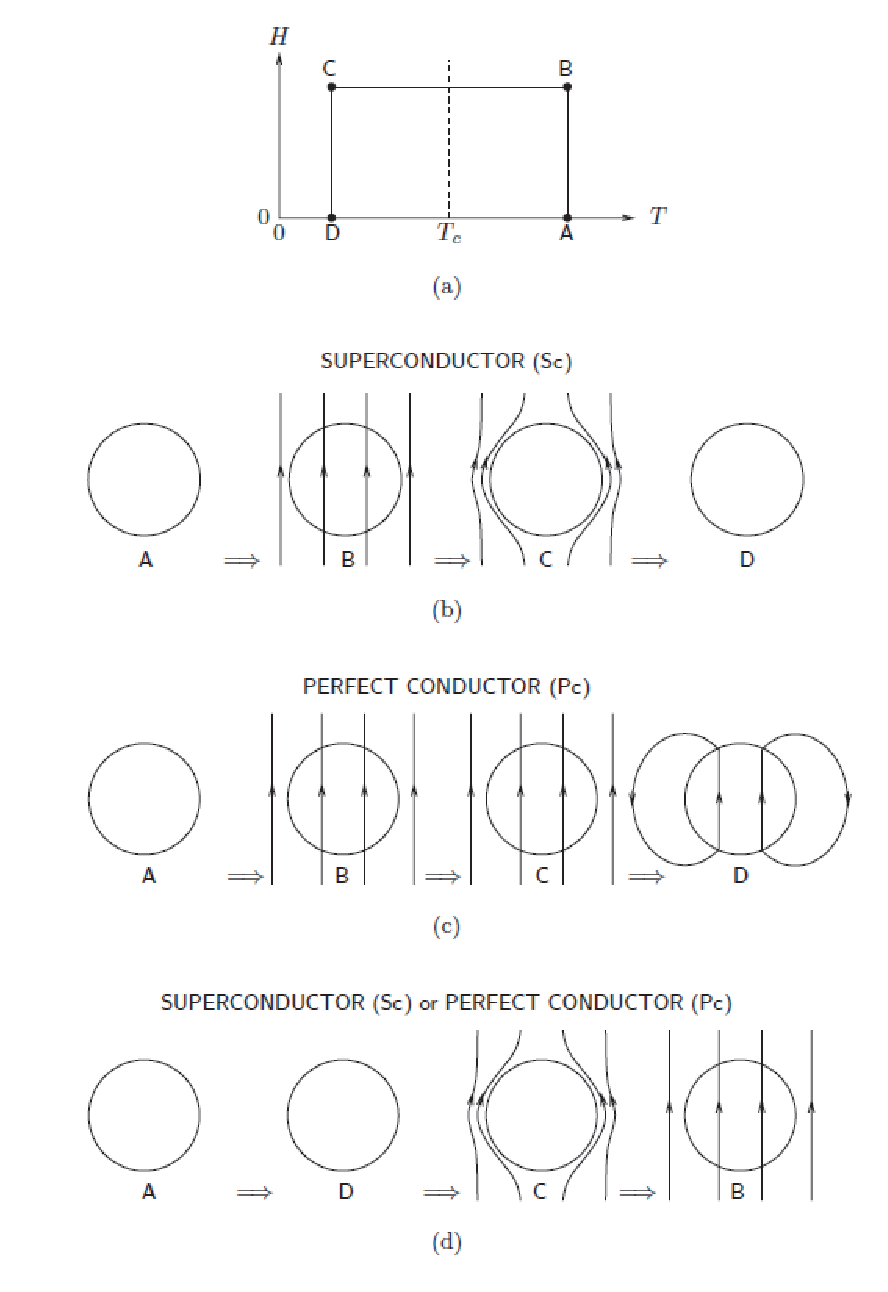
\includegraphics[scale=0.7]{chpt1/figs/fig1.1.eps}
  \caption{
(a): 两个球在$T <T_c$时的H-T相图,其中一个是超导体,另一个是理想导体。
(b): 超导球按$ A\rightarrow B\rightarrow C\rightarrow D$顺序施加H-T环境的磁场情况。
(c): 理想导体按相同的顺序施加H-T环境的磁场情况。
(d): 超导体或理想导体按$A\rightarrow D\rightarrow C\rightarrow B$顺序施加H-T环境的磁场情况。}
\end{figure}

\subsection{超导电性的London理论}
超导电性的唯象理论自1930年代开始发展(微观理论——BCS理论则是到1957年才完成的)。其中,London电磁理论
(1935年)提出“穿透深度”的概念来解释Meissner效应。简单的说,超导体被穿透深入为$\lambda$的表面超导电流
完全屏蔽了外磁场。根据London理论,$\lambda$由下式给出:
\begin{equation}
\lambda=\sqrt{\frac{m}{\mu_0 e^2 n_{se}}}
\end{equation}

式中,$m$和$e$分别是电子质量($9.11\times 10^{-31}\ \mathrm{kg}$)和电荷量($1.60\times 10^{-19}\ \mathrm{C}$);$\mu_0$是自由
空间磁导率($4\pi \times 10^{-7}\ \mathrm{H/m}$)。这里,超导电子密度$n_{se}$与自由电子$n_{fe}$不同。在$T=0$时,
全部都是超导电子;在$T=T_c$时,为零。定量地,有:
\begin{equation}
n_{se}\approx n_{fe}=\frac{\rho N_A}{W_A}
\end{equation}

其中,$\rho$是导体的质量密度($\mathrm{g/cm^3}$),$N_A$是Avogadro常数($6.023\times 10^{23}/\mathrm{mole}$),$W_A$是
原子质量($\mathrm{g/mole}$)。超导电流密度$J_c=e n_{se} v\approx e n_{fe} v$,$v$是超导电子的漂移速度。

\subsection{第I类和第II类超导体}
1911年,Onnes在纯汞中发现了超导电性;随后,其他金属如铅、锡也被发现是超导体。这些材料,现在被称为第I类超导体。
因其$H_c$较小(0.1 T),并不适合做超导磁体的材料。磁体级超导体属第II类。溯其源,第II类超导体由Haas和Voogd于
1930年在铅铋合金中发现。

第II类超导体可以用第I类超导体和正常导体材料的混合态来建模。1960年代初,有两种混合态物理模型:薄层模型(lamina)和岛模型(island)。
薄层模型是Goodman提出的,他认为第II类超导体的超导层被正常态层分割开。岛模型是Abrikosov提出的,不久得到了Essmann和Trauble的实验证实。
该理论认为在超导“海”中存在许多正常态的“岛”。对于第II类超导体,若要在0.1T以上还能保持超导态,正常态“岛”的半径必须小于$\lambda$。岛
半径是空间参数——相干长度$\xi$,这个参数是Pippard在1953年引入的。

$\xi$定义了超导/正常态转变发生的距离。根据用于解释第II类超导体超导电性磁场性质的GLAG理论,如果$\xi < \sqrt{2}\lambda$,是第II类超导体;
如果$\xi >\sqrt{2}\lambda$,则是第I类超导体。对合金来讲,由于缩短了自由电子的平均自由程,$\xi$会减小。$\xi$反比于材料正常态的电阻率。
两种常用的磁体级合金——$NbTi$和$Nb_3Sn$——的室温正常态电阻率都比铜打出一个数量级。值得注意的是,所有HTS的$\xi$都远小于$\lambda$。

\subsubsection{DC和AC响应}
图\ref{acdccurrent}给出了三个超导棒的示意图。第I类(1.2a)和第II类(1.2b,1.2c)中的载流均小于其临界电流。在第I类超导体重,无论通过AC抑或DC,
电流都只在表面(London穿透深度)流过且无能量耗散。第II类超导体中,DC电流在整个棒体内流过,尽管有正常区,但不产生耗散。我们可以设想,
“超导电子”通过材料时“躲”开了正常态区域。从电路的观点看,我们可以认为这些有电阻的“岛”被周围的超导“海”短路掉了。当通过AC时,第II类
超导体是有损耗的,即存在电阻——尽管其有效电阻仍然比正常高导电金属小几个数量级。每一个正常态区域都包含磁通束,称为磁通量子(fluxoid)或
旋涡(vortices)。磁通束在时变磁场和/或电流下“流”动。此种耗散性磁通流动是第II类超导体交流损耗的主要来源。

\begin{figure}
  \centering
 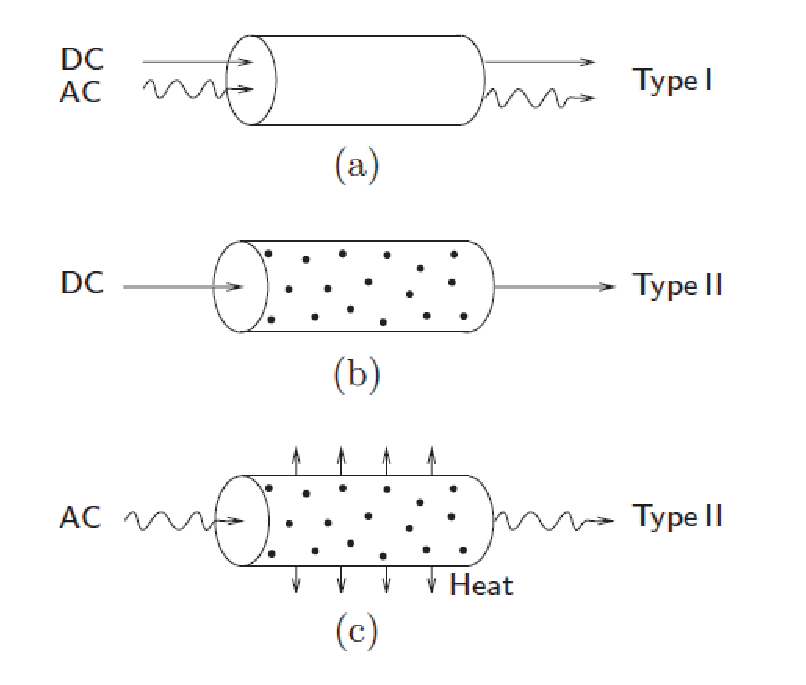
\includegraphics[scale=0.6]{chpt1/figs/fig1.2.eps}
  \caption{
超导棒载流。 (a) 第I类超导体棒, DC或AC电流——无焦耳耗散产生;
 (b) 第II类超导体棒,DC电流无耗散;(c) 第II类超导体棒,AC电流有焦耳热耗散产生。}\label{acdccurrent}
\end{figure}

\subsubsection{磁场性质}
置于磁场中,第I类超导体在$H<H_c$下是完全抗磁的,超过$H_c$就成为常规的无磁材料;第II类超导体在下磁场$H_{c1}$下,磁场性质和第I类一样,在$H_{c1}$和$H_{c2}$
之间时,第II类超导体是混合态。图\ref{mhcurve}给出了第I类/第II类超导体的磁化与磁场的关系。注意,磁体级超导体的磁化曲线都是不可逆的,并非如图中一样。不可逆的结果
就是存在磁滞曲线。第II类超导体的磁滞本性是其交流损耗的又一来源。

%%磁化曲线
\begin{figure}
  \centering
 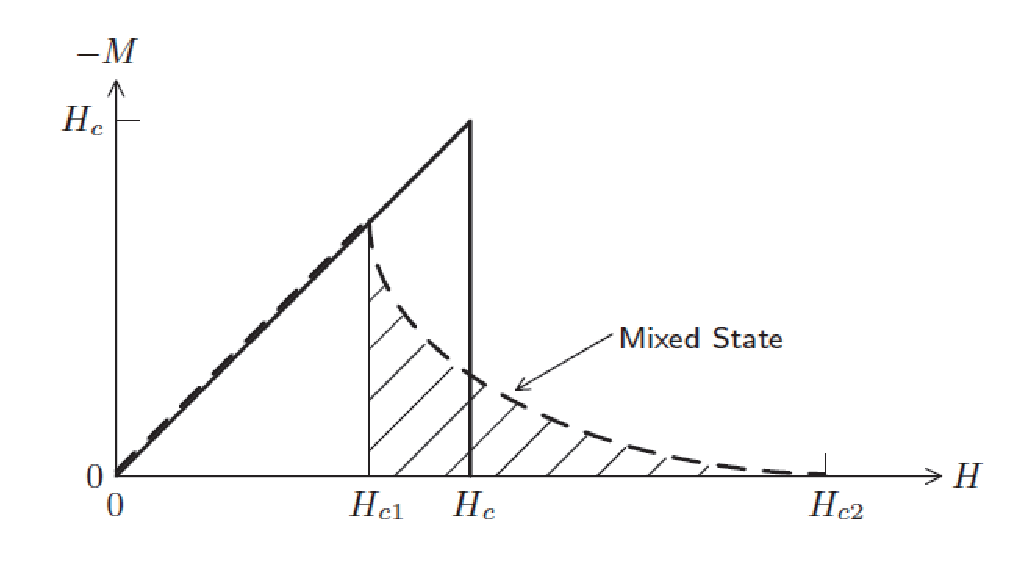
\includegraphics[scale=0.6]{chpt1/figs/fig1.3.eps}
  \caption{
M-H关系。实现是第I类,虚线是第II类。斜线区域表示第II类超导体的混合态。
}\label{mhcurve}
\end{figure}

\subsubsection{超导体举例}
表\ref{criticalparameters}列出了一些超导体,并给出了其类型、零场临界温度$T_c$、临界磁感应强度(第I类:$\mu_0H_c$;第II类:$\mu_0H_{c2}$)。所有的第I类超导体都是金属,临界场很小。
这也就解释了为什么Onnes在1913年试图用铅线做磁体会失败:在磁场下,铅就已经不超导了。即使那个时代,磁场也要达到0.3 T才有使用价值。表\ref{criticalparameters}已经很清楚的表明,
超导磁体必须使用第II类超导体。和第I类不同,第II类超导体存在多种类型:合金、金属混合物甚至氧化物。所有的氧化物都是高温超导体。$MgB_2$是非金属,也被
归为高温超导体。图\ref{tcvsyear}给出了几种代表性的HTS或LTS的$T_c$及其发现年份。图中还标出了重要制冷工质的沸点。其中,实线把氧化物超导体连缀了起来,虚线把金属类超导体
连缀了起来。

\begin{table}[htbp]\small%%表1.2
  \centering
  \caption{几种代表性第I类和第II类超导体的临界温度和临界磁场} \label{criticalparameters}
  \begin{tabular}{|l|c|c||l|c|c|}
    \hline
    % after \\: \hline or \cline{col1-col2} \cline{col3-col4} ...
    第I类 & $T_c[K]$ & $\mu_0 H_c[T]$ & 第II类 & $T_c[K]$ & $\mu_)H_c[T]$ \\ \hline \hline
    Ti & 0.39 & 0.0100 & Nb金属 & 9.5 & 0.2 \\ \hline
    Zr & 0.55 & 0.0047 & NbTi合金 & 9.8 & 10.5 \\ \hline
    Zn & 0.85 & 0.0054 &NbN & 16.8 & 15.3 \\ \hline
    Al & 1.18 & 0.0105&MgB2 & 39.0 & 35-60\\ \hline
    In & 3.41 & 0.0281 & Nb3Sn & 18.2 & 24.5  \\ \hline
    Sn & 3.72 & 0.0305  & Nb3Al & 18.7 & 31\\ \hline
    Hg & 4.15 & 0.0411  & Nb3Ge & 23.2 & 35.0\\ \hline
    V & 5.38 & 0.1403& YBCO & 93 & 150\\ \hline
    Pb & 7.19 & 0.0803 & Bi-22xx & 85-110 & >100 \\
    \hline
  \end{tabular}
\end{table}


\begin{figure}%%图1.4
  \centering
 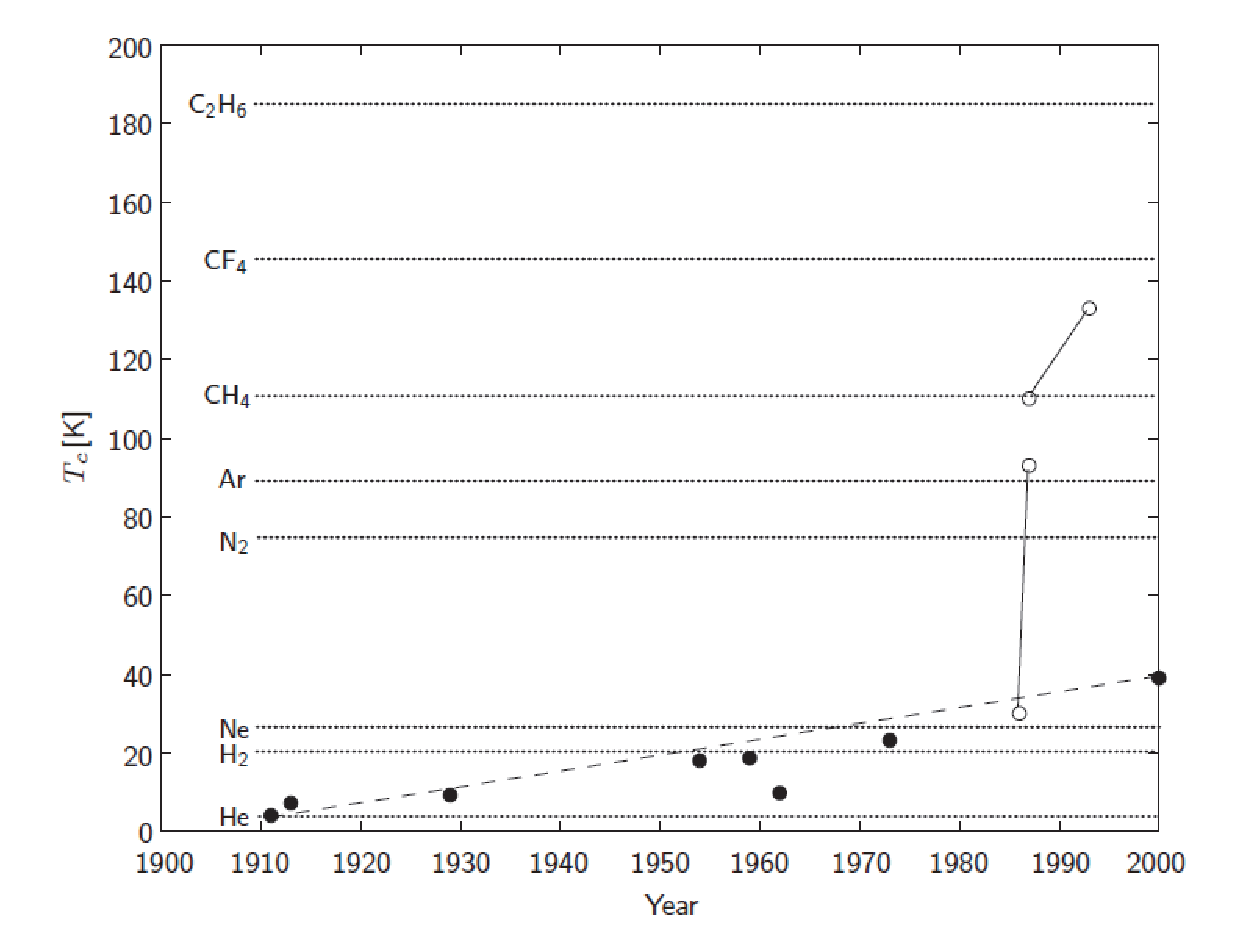
\includegraphics[scale=0.6]{chpt1/figs/fig1.4.eps}
  \caption{
几种代表性超导体$T_c$和发现年份
}\label{tcvsyear}
\end{figure}


\subsection{第II类超导体的临界面}
图\ref{ciriticalsurface}展示了一种典型的第II类磁体级超导体的临界面。超导电性存在于由边界函数$f_1,f_2,f_3$所确定的临界面之下。对磁体工程师更有用的,是一般的$f(H,T,J)$函数。
\begin{figure}
  \centering
 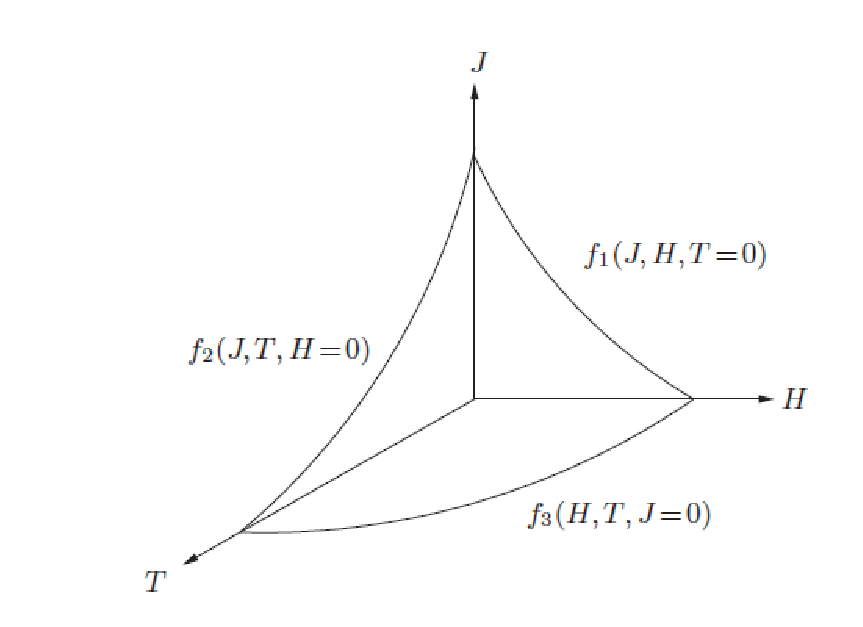
\includegraphics[scale=0.6]{chpt1/figs/fig1.5.eps}
  \caption{
典型第II类超导体的临界面
}\label{ciriticalsurface}
\end{figure}

\subsubsection{临界电流密度,$J_c$}
对第II类超导体,$J_c$可以通过冶金处理的方式大大提高。这种增强的$J_c$性能通常归因于“钉扎中心”的产生,钉住了旋涡,从而可以抵抗施加于其上的
Lorentz力($\vec{J}_c\times \vec{B}$)。这些晶体中的钉扎中心可通过材料掺杂、冶金处理(如冷处理产生错位,热处理产生前位体和晶界)等产生。Kim等给出:
\begin{equation}
  J_c\approx \frac{\alpha_c}{H+H_0}\
\end{equation}

式中,$\alpha_c, H_0$是常数。$\alpha_c$是$H\gg H_0$时平衡掉Lorentz力密度的渐近力密度。

\section{磁体级超导体}
磁体级超导体是指那些满足严格的磁体参数要求且可商业化取得的导体。以下是对磁体级超导体和超导材料的简短评论:现今每一种成功的磁体级超导体,都经历了长期和复杂的发展过程,才
从实验室走出,达到磁体级。
%%表1.3
\begin{table}[htbp]\small
  \centering
  \caption{超导材料 vs. 导体} \label{scmaterialvsconductor}
\begin{tabular}{|l|c||l|c|}
  \hline
  % after \\: \hline or \cline{col1-col2} \cline{col3-col4} ...
  标准 & 数量 & 标准 & 数量 \\ \hline \hline
  1.超导吗? & ~10000 & 3.$J_c>1\mathrm{GA/m^2}$? & ~10 \\ \hline
  2.$T_c> 4.2\mathrm{K};\mu_0 H_{c2}>10\mathrm{T}$? &~100 & 磁体级? & <10 \\
  \hline
\end{tabular}
\end{table}

\subsection{材料 vs. 磁体级超导体}
表\ref{scmaterialvsconductor}给出了满足特定标准的材料数量。随着标准推向磁体级,数量急剧减少。实际上,当今发现的10000多种超导体中,仅有几种可用于超导磁体。它们包括低温的$NbTi$、$Nb_3Sn$;
高温的Bi-2212、Bi-2223、涂层YBCO以及$MgB_2$。

\subsection{实验室超导体 vs. 磁体级超导体}
超导材料从实验室发现到磁体级,要经过很长的一段历程。可分为六个阶段:
\begin{enumerate}
  \item 发现;
  \item 提高$J_c$性能
  \item 与基底金属的共处理;
  \item 多丝成形;
  \item $I_c>100\ \mathrm{A}$且长度$>1000\ \mathrm{m}$;
  \item 其他要求,如强度和应力容许值。
\end{enumerate}

表\ref{scstage}给出了$Nb_3Sn$和Bi-2223的六个阶段开始的大致时间。值得注意的是,Bi-2223最开始是与常规金属银共处理的。阶段2一直持续到今天。对于涂层YBCO,目前大致处于
阶段3晚期,即将进入阶段4。目前已经有了使用YBCO制作的运行于77K的小线圈。2001年发现的$MgB_2$已经进入阶段5,目前已有“大”$MgB_2$磁体建成投运。

1961年,发现$Nb_3Sn$。尽管之后经过十多年的紧张R\&D,到现在应用于多数磁体时,仍需由用户自定制性质。因其脆性和应力承受不能超过$~0.3\%$,在本质上是不易处理的,需要战战兢兢。
BSCCO与此情形很类似。
%表1.4
\begin{table}[htbp]\small
  \centering
  \caption{$Nb_3Sn$和$Bi-2223$从材料到导体的发展阶段} \label{scstage}
\begin{tabular}{|c||l|l|l|}
  \hline
  % after \\: \hline or \cline{col1-col2} \cline{col3-col4} ...
  阶段&事件& $Nb_3Sn$ &$Bi-2223$ \\ \hline \hline
1 & 发现 & 1950年代早期& 1980年代晚期 \\ \hline
2 & 实现短样大$J_c$ & 1960年代早期 & 1990年代早期\\ \hline
3 &与基底金属共处理&1960年代晚期&1990年代早期\\ \hline
4 &多丝成形&1970年代早期&1990年代中期\\ \hline
5 &$I_c\ge 100\ \mathrm{A}$;长度$\ge 1000\ \mathrm{m}$ &1970年代中期&2000年代早期\\ \hline
6 &其他磁体需求&1970年代晚期&2000年代中期\\
  \hline
\end{tabular}
\end{table}


\section{磁体设计}
\subsection{要求和关键}
无论用于实验还是作为系统的组件,磁体都必须满足磁场的基本要求:规定的空间分布和时间变化特征。磁场的规格常由以下重要参数给定:1. $H_0$,磁体中心($x=0, y=0, z=0$)场强;
2.$V_0$,规定磁场的体积;3.$H(t)$,磁场的时变性。1和3,将在第二章和第三章详细讨论。

除了满足上述基本要求,磁体设计还必须处理以下关键点:
\begin{description}
  \item[机械完整性] 磁体必须有足够的结构强度,承受正常运行和故障时的巨大磁场应力。
  \item[运行可靠性] 磁体必须稳定、可靠的达到并维持于工作点。磁体的这种稳定性,一般简称为磁体稳定性。运行中磁体失去超导电性的过程叫\textbf{“失超”}。
  \item[保护] 磁体一旦发生可能引起其进入正常态的事件,必须能保证不被损坏并且(能在事件解除后)能再次上电且运行在工作点上。
  \item[导体] 对量产的磁体,超导磁体系统的费用很大程度上受超导体费用的影响。即导体费用决定磁体费用。本书很少定量处理有关多种方案经济性选择的导体费用问题,比如
$NbTi@1.8\ \mathrm{K}$,$Nb_3Sn@4.2\ \mathrm{K}$,$NbTi@4.2\ \mathrm{K}$,$MgB_2@15\ \mathrm{K}$。
  \item[制冷] 由于磁体运行需要能量来创造并维持低温环境,故制冷成为超导磁体的一个重要问题。制冷对于整个系统的重要性常被过分强调。这里必须指出,哪怕在很多超导磁体是作为关键部件的应用
  中,磁体不过是整个系统的一个组件,而制冷又是磁体组件的子组件。制冷系统的功劳需求通常仅占整个系统的一个很小的份额。
\end{description}

磁体的终极发展目标是市场化。若想取得成功,还需要加入两个要素:1.价格;2.易用性。

\subsection{运行温度的影响}
LTS磁体的基本温度通常是4.2 K。仅HTS磁体可能运行于高于4.2 K的温度。运行温度影响到磁体的5个方面:机械完整性、稳定性、保护、导体和制冷。图1.6给出了“难度或费用”与运行温度的定性关系。
%图1.6
\begin{figure}
  \centering
 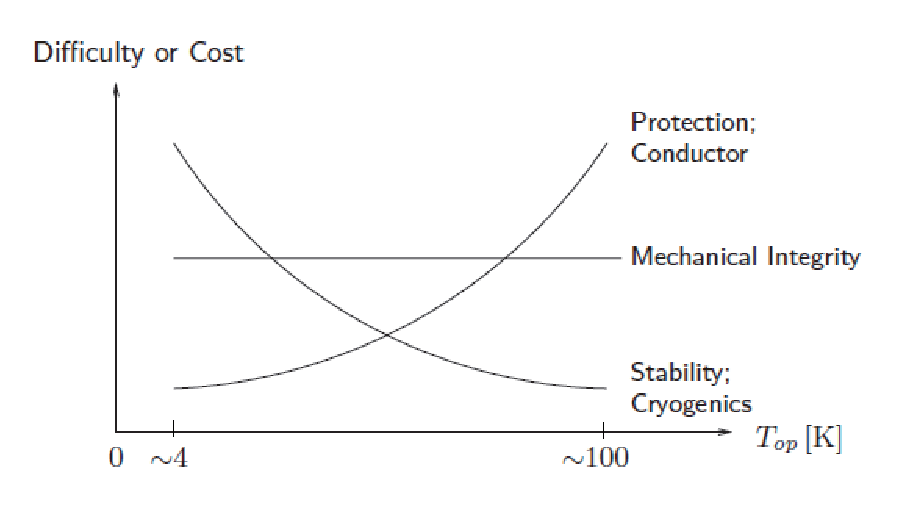
\includegraphics[scale=0.6]{chpt1/figs/fig1.6.eps}
  \caption{
温度对磁体的五个关键点的影响
}\label{temperatureeffect}
\end{figure}
LTS的温区通常是1.8-10\ K,HTS的温区一般是20-80\ K。对于LTS/HTS混合系统,运行温度由LTS决定,即<10\ K。图\ref{temperatureeffect}中,保护与导体、稳定性与制冷用同一条曲线仅表示趋势,并不代表实际上的重合。

图\ref{temperatureeffect}表明,机械完整性的要求基本与运行温度无关。这个结论对运行温度到~100K都是适用的。在这个温区范围内,磁体的不同材料的热膨胀都是可忽略的。对于一个给定磁场要求的磁体,必要安匝数
与运行温度基本无关。因为已知的超导体都是随温度上升,临界电流密度下降。导体费用总是随温度上升而提高:降低制冷费用的期望收益一定要与导体费用的增加值作比较。运行稳定性和保护受运行温度影响较大。

\section{数值解}
如本书开始所指出的,超导磁体技术是跨学科的,需要精炼的机械、电气、制冷和材料领域的专业知识。其实这也意味着,一个人是不可能完成满足每一个实际磁体设计和运行参数需求的可靠的数值解的。
通常,需要一个专业的团队来做成此事。
\subsection{粗算解}
制冷工程师或其他成员没必要对磁场专家的所有磁场计算深信不疑。制冷专家应当能够计算相对复杂条件下的大致磁场。本书的一个目标就是让设计团队的每一个成员都具备在自己领域以及其他领域
进行粗算的能力。实际上,每一个新磁体系统都应这样开始:每一个成员都来对每一个重要的设计和运行参数粗算一遍。而后,磁体制造和运行的更精确的数值由组内领域专家计算。

\subsection{程序解}
对磁体系统的实际制造和运行,每一个设计和运行参数一般都必须采用程序辅助计算。多数设计团队使用ANSYS、VectorFields、COMSOL。几种软件都可用于磁场、应力应变以及热的分析。
专用程序,例如GANDALF、THEA专门用于处理CICC导体构成的大型磁体,特别是聚变磁体的失超发生和传播现象。失超现象包含热、流体、电暂态、电缆和工质的变化很大,热物理和电性质的变动幅度跨越1-2个数量级。正是这个原因,失超暂态多(有时完全是)依赖于数值仿真。数值仿真能处理非线性热发生和热传导,以及工质的热诱导的可压缩黏性流动。上述每一套程序都是基于超过25年的大量
专家的工作。

GANDALF和THEA都是商业软件。GANDALF最初是用来分析ITER导体的热-流体暂态的。THEA的主要特征是将热、流体模型扩展到多平行通道。
%【此句不通】如多丝具有不同温度,平行流通道,包括非均一电流分布和暂态重分配。

\section{专题}
\subsection{问题1.1:第I类超导体的热力学性质}
第I类超导体的单位体积比热($\mathrm{J/m^2K}$)由下式给出:
\begin{subequations}\label{eqn:1.4ab}
	\begin{align}
\mbox{超导态:} C_s(T) &= aT^3 \\
\mbox{正常态:} C_n(T)&= bT^3+\gamma T	
	\end{align}
\end{subequations}

式中,$a,b,\gamma$都是常数。

a)证明零场时的转变温度为:
\begin{equation}\label{eqn:1.5}
  T_c=\sqrt{\frac{3\gamma}{a-b}}
\end{equation}

可采取下列步骤:1)熵的表达式$C(T)=T\partial S(T)/\partial T$;2)注意到$H=0$时,有$S_n(T_c)-S_s(T_c)=0$。

b)证明$H_{c0}$在$T=0K, H_{c0}\equiv H_c(0)$时,由下式给出:
\begin{equation}\label{eqn:1.6}
  H_{c0}=T_c \sqrt{\frac{\gamma}{2\mu_0}}
\end{equation}

证明临界磁场$H_c(T)$是$T$的二次函数:
\begin{equation}\label{eqn:1.7}
  H_c(T)=H_{c0}\left[1-(\frac{T}{T_c})^2\right]
\end{equation}

注意到零场时单位体积的吉布斯自由能关系:
\begin{equation}\label{eqn:1.8}
  G_n(T)-G_s(T)=\frac{1}{2}\mu_0 H_c^2(T)
\end{equation}

根据方程1.8以及$S(T)=-\partial G(T)/\partial T$,可以推导出方程1.6。

c)证明内能密度差$U_n-U_s$在自场下于$T_{ux}$时取最大:
\begin{equation}
  T_{ux}=\frac{T_c}{\sqrt{3}}
\end{equation}

注意到,在零场时有:$U(T)=\int C(T)dT$

d)缓慢绝热施加磁场(初始温度为$T_i$,$0<T_i<T_c$),磁场加至略大于临界值,此时相变至正常态,降低导体温度到$T_j (<T_i)$。给出$T_i$和$T_j$的关系,并
画出本过程的热力学相图。

e)对于同一个初始温度为$T_i$($0<T_i<T_c$)的超导体,位于零场中突然施加$H_e$,如果$H_e$超过临界值$H_{ec}$,材料将被加热,证明
\begin{equation}
  H_{ec}(T_i)=H_c(T _i)\sqrt{\frac{1+3(T_i/T_c)^2}{1-(T_i/T_c)^2}}
\end{equation}

\subsubsection{问题1.1之解答}
a) 由于$C(T)=TdS(T)/dT $以及$S(T = 0)=0$,我们有
 $$S(T) =\int_{0}^{T}C(T)dT \eqno (S1.1) $$

将\ref{eqn:1.4ab}代入上式,有:
$$S_s(T) =\int_{0}^{T}\frac{C_s(T)}{T}dT=\frac{1}{3}aT^3 \eqno (S1.2a)$$
$$S_n(T) =\int_{0}^{T}\frac{C_n(T)}{T}dT = \frac{1}{3}bT^3 + \gamma T \eqno (S1.2b)$$

于是,
$$S_n(T) − S_s(T) =\gamma T − \frac{1}{3} (a − b)T^3 \eqno (S1.3)$$

由于上面已经指出,在$H=0$时,有$S_n(T_c)−S_s(T_c)=0$,所以,
$$\gamma= \frac{1}{3} (a − b)T^2 \eqno (S1.4)$$

解出$T_c$,有
$$T_c=\sqrt{\frac{3\gamma}{a-b}}\eqno (1.5)$$

b) 从式\ref{eqn:1.8}以及$S(T)=−\partial G(T)/\partial T$,我们有
$$S_n(T) − S_s(T) = −\mu_0 H_c(T)\frac{\partial H_c(T)}{\partial T} \eqno (S1.5)$$

联立S1.3和S1.4,重写$(a-b)/3=\gamma/T_c^2$,我们有
$$S_n(T) − S_s(T)=\gamma T\left[1-\left(\frac{T}{T_c}\right)^2\right] \eqno (S1.6)$$

联立上面粮食,对T积分,有
$$−\frac{1}{2}\mu_0 H_c^2(T) =\frac{1}{2}\gamma T_c^2-
\frac{1}{4}\gamma T_c^2 \left(\frac{T}{T_c}\right)^4+A \eqno (S1.7)$$

式中,A是常数。由于$H_c(T =0)\equiv H_{c_0}$,我们有$A=−\mu_0 H_{c_0}^2 / 2$。在
$T=T_c$时,由于$H_c(T_c)=0$,上式成为
$$0=\frac{1}{2}\gamma T_c^2-\frac{1}{4}\gamma T_c^2-\frac{1}{2}\mu_0 H_{c_0}^2 \eqno (S1.8)$$

解出$H_{c_0}$,有
$$H_{c_0}=T_c\sqrt{\frac{\gamma}{2\mu_0}}\eqno (1.6)$$

从上式,我们可以得到
$$\gamma=\frac{2\mu_0 H_{c_0}^2}{T_c^2} \eqno (S1.9)$$

联立S1.7和上式,得到
$$-\frac{1}{2}\mu_0 H_c^2(T)=\mu_0 H_{c_0}^2 (\frac{T}{T_c})^2-\frac{1}{2}\mu_0 H_{c_0}^2 (\frac{T}{T_c})^4-\frac{1}{2}\mu_0 H_{c_0}^2  \eqno (S1.10)$$

上式可以重写为:
$$H_c^2(T)=H_{c_0}^2\left[1-2(\frac{T}{T_c})^2+(\frac{T}{T_c})^4\right]=H_{c_0}^2\left[1-(\frac{T}{T_c})^2\right]^2 \eqno (S1.11)$$

从上式,我们可以得到:
$$H_c(T)=H_{c_0}\left[1-\frac{T}{T_c}\right]\eqno (1.7)$$

由\ref{eqn:1.6},我们可以根据第一类超导体实验测得的$\gamma$和$T_c$计算预测$H_{c_0}$。下表给出了通过公式
计算和实测的$\mu_0 H_{c_0}$数据。同时还给出了一些其他实测数据。
%表1.5
\begin{table}[htbp]\small
  \centering
  \caption{$H_{c_0}$:公式\ref{eqn:1.6}计算值和实测值} \label{tb:eqn1.6andexp}
\begin{tabular}{|c||c|c|c|c|c|c|}
  \hline
  % after \\: \hline or \cline{col1-col2} \cline{col3-col4} ...
超导体&$\rho [\mathrm{g/cm^3}]$&$M [\mathrm{g/mole}]$&$\gamma [\mathrm{J/m^3K^2}]$&$T_c [\mathrm{K}]$&$\mu_0 H_{c_0}$计算&$\mu_0 H_{c_0}$实测 \\ \hline \hline
Ti&4.53&47.88&316.8&0.39&5.6&10.0 \\ \hline
Zr&6.49&91.22&199.2&0.55&6.1&4.7\\ \hline
Zn&7.14&65.38&69.8&0.85&5.6&5.4\\ \hline
Al&2.70&26.98&135.1&1.18&10.9&10.5\\ \hline
In&7.31&114.8&107.6&3.41&28.0&28.1\\  \hline
Sn&7.31&118.7&109.6&3.72&30.9&30.5\\  \hline
Hg&13.55&200.6&120.9&4.15&36.2&41.1\\  \hline
V&6.11&50.94&1111&5.38&142.7&140.3\\  \hline
Pb&11.35&207.2&163.2&7.19&72.8&80.3 \\  \hline
\end{tabular}
\end{table}

c) 由零场时的$dU(T)=C(T)dT$,我们可以得到
\begin{equation*}
U(T) =\int_{0}^{T}C(T) dT  \tag{S1.12}
\end{equation*}

代入式\ref{eqn:1.4ab},得到
\begin{equation*}
U_n(T) =\int_{0}^{T}(bT^3 +\gamma T)dT = \frac{1}{4}bT^4 +\frac{1}{2}\gamma T^2 \tag{S1.13a}
\end{equation*}
\begin{equation*}
U_s(T)=\frac{1}{4}aT^4 \tag{S1.13b}
\end{equation*}

两个自由能的差表示为:
\begin{equation*}
\begin{split}
U_n(T) − U_s(T) =&\frac{1}{4} (b − a)T^4 + \frac{1}{2}\gamma T^2\\
=&\left(\frac{a-b}{4}\right)\left[\frac{2\gamma}{a-b}T^2-T^4\right]
\end{split} \tag{S1.14}
\end{equation*}

对上式微分,并在$T=T_{ux}$处令其为零,有:
\begin{equation*}
\frac{d(U_n-U_s)}{dT}|_{T_{ux}}=\frac{a-b}{4} \left[\frac{4\gamma}{a-b}T_{ux}-4T_{ux}^3\right]=0 \tag{S1.15}
\end{equation*}

于是
\begin{equation*}
\frac{4\gamma}{a-b}T_{ux}-4T_{ux}^3=0 \tag{S1.16}
\end{equation*}

利用\ref{eqn:1.5},解出$T_{ux}$,可得
\begin{equation*}
T_{ux}=\sqrt{\frac{\gamma}{a-b}}=\frac{T_c}{\sqrt{3}} \tag{1.9}
\end{equation*}

d) 由于这个过程是绝热和可逆的,那么如果场是缓慢施加的,有$S_n(T)=S_s(T)$。从S1.2可以得到
\begin{equation*}
S_n(T_f ) − S_s(T_i) =\frac{1}{3}bT_f^3 +\gamma T_f −\frac{1}{3}aT_i^3 \tag{S1.17}
\end{equation*}

由$S_n(T_f )−S_s(T_i)=0$,我们得到关于$T_f$和$T_i$的表达式
\begin{equation*}
\frac{1}{3}bT_f^3 +\gamma T_f =\frac{1}{3}aT_i^3 \tag{S1.18}
\end{equation*}

从\ref{eqn:1.5},我们有
\begin{equation*}
b = a − \frac{3\gamma}{T_c^2} \tag{S1.19}
\end{equation*}

联立上面两式,有
$$\frac{1}{3}a(T_f^3-T_i^3)=-\gamma T_f\left[ 1-\left(\frac{T_f}{T_c}\right)^2\right] \eqno (S1.20)$$

由于$T_f<T_c$,上式的右侧是负值,于是可知$T_f<T_i$。图1.7给出了超导态(实线)和正常态(虚线)
的T-S图。$T_i\rightarrow T_f$转变在途中用竖实线表示。
\begin{figure}
  \centering
 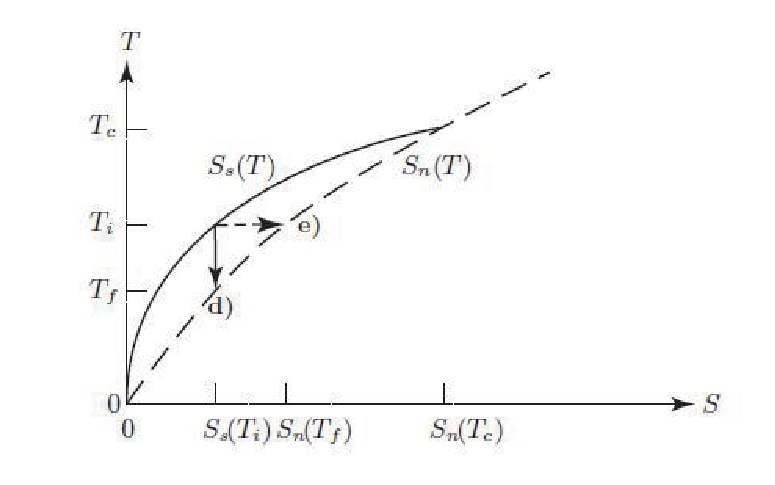
\includegraphics[scale=0.7]{chpt1/figs/fig1.7.eps}
  \caption{超导态(实线)和正常态(虚线)的T-S图}\label{fig:tsplot}
\end{figure}

e) 超导体被加热,首先必须先进入正常态。外场需提供磁场能$\mu_0 H_c^2(T_i)/2$。由于转变过程要吸热
$T_i[S_n(T-i)-S_s(T_i)]$,故还必须提供吸收能$H_{ec}$。图\ref{fig:tsplot}中的虚横线就是转变过程。于是,
$$\frac{1}{2}\mu_0 H_{ec}^2(T_i)=\frac{1}{2}\mu_0 H_c^2(T_i)+T_i[S_n(T-i)-S_s(T_i)] \eqno (S.1.21)$$

上式和S1.1联立,得到
$$\frac{1}{2}\mu_0 H_{ec}^2(T_i)=\frac{1}{2}\mu_0 H_c^2(T_i)+T_i[\frac{1}{3}(b-a)T_i^3+\gamma T_i] \eqno (S1.22)$$

把S1.9代入上式,并应用S1.19,得到
$$\frac{1}{2}\mu_0 H_{ec}^2(T_i)=\frac{1}{2}\mu_0 H_c^2(T_i)+2\mu_0 H_{c_0}^2\left(\frac{T_i}{T_c}\right)^2 \left[1-\left(\frac{T_i}{T_c}\right)^2 \right]\eqno (S1.23)$$

联立式\ref{eqn:1.7},得到
$$H_{ec}^2(T_i)=H_c^2(T_i)+4H_c^2(T_i)\frac{(T_i/T_c)^2}{1-(T_i/T_c)^2} \eqno (S1.24)$$

于是
$$H_{ec}(T_i)=H_c(T_i)\sqrt{\frac{1+3(T_i/T_c)^2}{1-(T_i/T_c)^2}}$$

由于$H_c(T_c)=0$,可知$H_{ec}(T_c)=0$;另有$H_{ec}(T_i)\ge H_c(T_i)$。


\subsection{问题1.2:超导回路}
本问题表明不可能通过外施电流源的方法在闭合超导回路、线圈或盘中产生持续电流。
此处用电路模型证明,参数如图\ref{scloop}。

a)写出两个回路的电路方程。

b)解出$I_s(t)$,证明以一个开始和最后都是0的$I(t)$($I(t=0)=I(t=\inf)=0$)不能建立起闭合回路的电流。
闭合超导回路可能是一个通过超导部件连接了引线的磁体、超导饼、超导盘。

%图
\begin{figure}
  \centering
 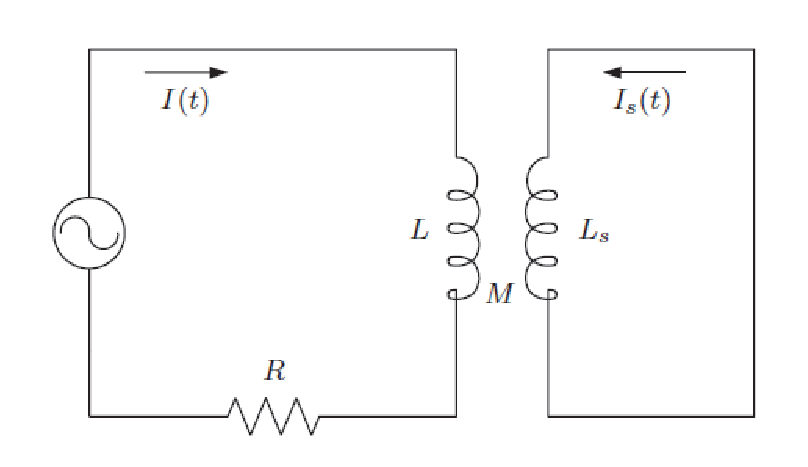
\includegraphics[scale=0.6]{chpt1/figs/fig1.8.eps}
  \caption{
超导线圈回路与一个带有电流源的回路通过电感耦合
}\label{scloop}
\end{figure}

\subsubsection{问题1.2之解答}
a) 两个电压方程为
$$L\frac{dI(t)}{dt}+M\frac{dI_s(t)}{dt}+ RI = 0 \eqno (S2.1a)$$
$$M\frac{dI(t)}{dt}+ L_s\frac{dI_s(t)}{dt}= 0 \eqno (S2.1b)$$

b)从S2.1b中可以解得
$$I_s(t) = −\frac{M}{L_s}I(t) + C  \eqno (S2.2)$$

因为$I_s(t=0)=0$,所以,$C=0$。由于$I(t=0)=I(t=\inf)=0$,所以仅在$I(t)\neq 0$时有$I_s(t)\neq 0$。
也即,在无外电流源也无初始值的超导回路不能孤立的维持能量。

在一个超导回路中不能产生感应电流在某些应用中是有实际意义的。持续运行模式的磁体必须通过引线通入电流
充电(处于驱动模式)。此后,通过所谓的“超导开关”(persistent current switch,PCS)将引线短路,电流源
可以去掉。


\subsection{问题1.3:磁共振成像(MRI)}
超导磁体最成功的商业应用之一便是医疗诊断装置,特别是MRI。以下是磁体工程师需要了解的一些基本问题:

a)MRI中,为什么$H^1$、$N^{14}$核可以被探测到,而$C^{12}$、$O^{16}$探测不到?

b)如果频率分辨率是$10\ \mathrm{Hz}$,对于1T全身MRI磁体的中心磁场均匀性最小要求多少?对全身MRI磁体,室温孔直径$80\ \mathrm{cm}$,这个均匀场区域通常在$25\ \mathrm{cm}$ DSU(直径半球体积)。

c)MRI单元中,脉冲梯度磁体的作用?

d)对1T磁体单元,脉冲磁体产生的典型$\frac{d\vec{B}}{dz}$是多少?

\subsubsection{问题1.3之解答}
a) 有奇数质子或中子的原子核存在净角动量。处于磁场中,原子核按某种正比于磁场强度的特定频率(Larmor)进动。
比如氢的Larmor频率在1T时是$42.576MHz$。表1.6\footnote{加粗的数字表示可探测}给出了几种物质原子的数据。
%表1.6
\begin{table}[htbp]\small
  \centering
  \caption{几种元素的原子核数据} \label{tb:atomic}
\begin{tabular}{|c||c|c|c|c|c|}
  \hline
  % after \\: \hline or \cline{col1-col2} \cline{col3-col4} ...
原子序数&元素&原子质量&质子数&中子数&可探测? \\ \hline \hline
1&氢&1&\textbf{1}&0&是 \\ \hline
6&碳&12&6&6&否 \\ \hline
6&碳&13&6&\textbf{7}&是 \\ \hline
7&氮&14&\textbf{7}&\textbf{7}&是 \\ \hline
8&氧&16&8&8&否 \\ \hline
11&钠&23&\textbf{11}&12&是 \\ \hline
15&磷&31&\textbf{15}&16&是 \\ \hline
\end{tabular}
\end{table}

b) 由于$10\ \mathrm{Hz}$相当于 $42.576×10^6\ \mathrm{Hz}$的$0.23×10^{−6}$,所以磁场必须是1T的$0.23×10^{−6}$ ,
大约是 $0.002\ \mathrm{gauss}$。作为对比,地磁场约为$0.7 \ \mathrm{gauss}$。

c) 通过引入特定的空间磁场分布,我们可以限制在某个制定区域产生共振。
这让我们可以对某一个特定核素进行成像。

d) 梯度幅值直接和成像的空间解析度相关。更高的梯度可以同比例产生更好的解析度。但存在一个磁体
和患者可以忍受的极限问题。医用MRI必须限制梯度强度——至少应限制梯度偏斜率——以避免产生对神经
和肌肉的刺激。医用MRI的最大梯度约为$3-4 \ \mathrm{gauss/cm}$,最大场偏斜率约为$12\ \mathrm{(gauss/cm)/ms}$或者
$120\ \mathrm{(T/m)/s}$。

